%!TEX root = ../thesis.tex

\subsection{軌道生成とは}

\begin{figure}[hbtp]
  \centering
 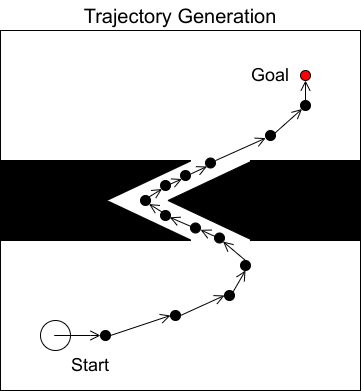
\includegraphics[keepaspectratio, scale=0.8]
      {images/png/TrajectoryGeneration.drawio.png}
 \caption{Trajectory Generation}
 \label{Fig:TrajectoryGeneration}
\end{figure}

軌道生成は,「1.1.1 経路と軌道の違い」で述べたように,ロボットがどのような運動で通るかを決めることである.
多くの経路計画ではロボットの運動学やメカニズムを無視しているため,ロボットの機構や特性で動作が難しい経路が計画されることがある.その例を以下に示す.
\begin{quote}
     \begin{itemize}
      \item アッカーマンリンクの自動車がその場で90°回転するような経路
      \item 対向二輪のロボットが姿勢を変えずに車輪に対して垂直に移動するような経路
      \item 等速で狭い場所も広い場所を通るような経路
     \end{itemize}
\end{quote}
そこで,ロボットが実際に動作及び制御可能な範囲で経路を追従させるために運動学やメカニズムを考慮した「軌道生成」を用いてロボットの運動
を決める.軌道生成を行うことで狭い道で速度を遅くしたり,広い道では速度を速くするといった動作や計画された経路の通過地点に対してロボットの機構や特性を
考慮した軌道を生成することができる.

Fig.\ref{Fig:TrajectoryGeneration}は軌道生成のイメージである.
黒い点がロボットの位置であり,矢印がロボットの速度,中央にある黒い部分が障害物である.
軌道生成ではこのようなロボットの軌道を生成することができる.
\newpage